\documentclass[12pt]{standalone}

%% for compilation with htlatex (to produce svg image),
%% uncomment the line below:
%\def\pgfsysdriver{pgfsys-tex4ht.def}

\usepackage{tikz}

\tikzstyle{tensor}=[rectangle,draw=blue!50,fill=blue!20,thick]
\tikzstyle{dots}=[thick]


\begin{document}

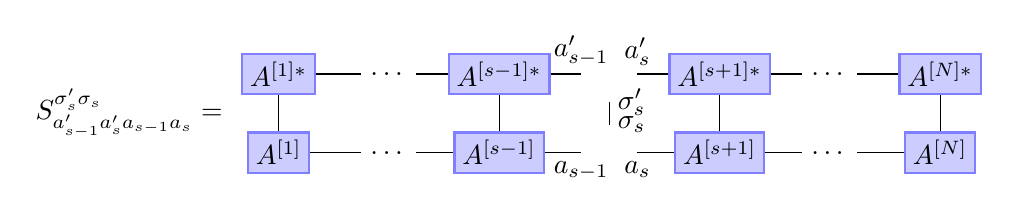
\begin{tikzpicture}[inner sep=1mm]
  \def\sep{1.4};
  %\def\x{1068}
  \node[tensor] (1 spin conjugate) at (\sep, 0.5) {$A^{[1]*}$};
  \node[tensor] (1 spin) at (\sep, -0.5) {$A^{[1]}$};
  
  \node[dots] (2 spin) at (2*\sep, -0.5) {\dots};
  \node[dots] (2 spin conjugate) at (2*\sep, 0.5) {\dots};

  \node[tensor] (3 spin) at (3*\sep, -0.5) {$A^{[s-1]}$};
  \node[tensor] (3 spin conjugate) at (3*\sep, 0.5) {$A^{[s-1]*}$};

  \node[minimum width=0.7cm, minimum height=0.7cm] (4 spin) at (4*\sep,-0.5) {};
  \node[minimum width=0.7cm, minimum height=0.7cm] (4 spin conjugate) at
    (4*\sep,.5) {};

  \node[tensor] (5 spin) at (5*\sep, -0.5) {$A^{[s+1]}$};
  \node[tensor] (5 spin conjugate) at (5*\sep, 0.5) {$A^{[s+1]*}$};

  \node[dots] (6 spin) at (6*\sep, -0.5) {\dots};
  \node[dots] (6 spin conjugate) at (6*\sep, 0.5) {\dots};

  \node[tensor] (7 spin) at (7*\sep, -0.5) {$A^{[N]}$};
  \node[tensor] (7 spin conjugate) at (7*\sep, 0.5) {$A^{[N]*}$};
  
  \foreach \x in {1,3,5,7} {
    \draw[-] (\x \space spin) -- (\x \space spin conjugate);
  }
  \foreach \x in {1,5} {
    \pgfmathtruncatemacro{\xplusone}{\x + 1};
    \pgfmathtruncatemacro{\xplustwo}{\x + 2};
    \draw[-] (\x \space spin) -- ({\xplusone \space spin}.west);
    \draw[-] (\x \space spin conjugate) -- ({\xplusone \space spin conjugate}.west);
    \draw[-] ({\xplusone \space spin}.east) -- (\xplustwo \space spin);
    \draw[-] ({\xplusone \space spin conjugate}.east) 
      -- (\xplustwo \space spin conjugate);
  }

  \draw (4 spin.north) node[right] {$\sigma_s$} -- (4 spin conjugate.south)
  node[right] {$\sigma_s'$};
  \draw (3 spin) -- (4 spin.west) node[below] {$a_{s-1}$};
  \draw (5 spin) -- (4 spin.east) node[below] {$a_{s}$};
  \draw (3 spin conjugate) -- (4 spin conjugate.west) node[above] {$a_{s-1}'$};
  \draw (5 spin conjugate) -- (4 spin conjugate.east) node[above] {$a_{s}'$};

  \node at (-.5, 0.) {$S_{a_{s-1}'a_s' a_{s-1}a_s}^{\sigma_s' \sigma_s} = $};
    %\draw[-] (1.west) .. controls +(-1.5, 1) and +(1.5, 1) .. (5.east);
\end{tikzpicture}

\end{document}

